\section{Propagaci\'on del Error Experimental}

\subsection{Objetivo}
Determinar el error y su propagación por medio de experimentos, al usar distintos instrumentos de medición.

\subsection{Fundamento te\'orico}
\begin{itemize}
    \item \textbf{Medir}: Una medición es comparar la cantidad desconocida que queremos determinar y una cantidad conocida de la misma magnitud, que elegimos como unidad. Al resultado de medir se le denomina medida.
    \item \textbf{Instrumentos de medición}: Es un instrumento que se usa para medir una cantidad física. Los instrumentos de medición se caracterizan por su precisión, exactitud, resolución, apreciación, sensibilidad.
    \item \textbf{Error}: El error de medición es la diferencia que hay entre el valor medido y el valor real. Este puede deberse a diversas causas, entre ellas están los factores ambientales, desgaste o fallo en el diseño del instrumento.
    \item \textbf{Propagación de error}: Es el efecto de variables de incertidumbre en la incertidumbre de una función matemática basada en ellos. Cuando las variables son los valores de mediciones experimentales tienen incertidumbre debido a la medición de limitaciones (por ejemplo, instrumento de precisión), que se propagan a la combinación de variables en la función.
\end{itemize}

\subsection{Materiales}

\begin{figure}[H]
	\begin{center}
 		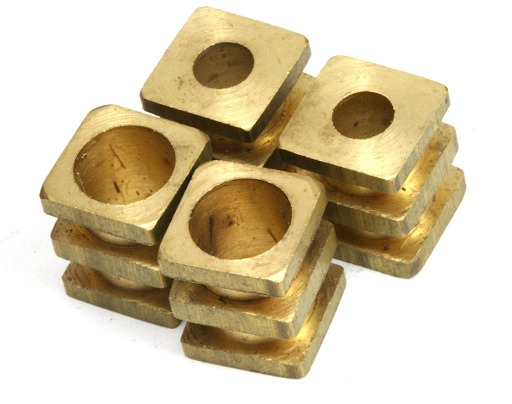
\includegraphics[width = 0.3\textwidth]{Imagenes/para.jpg}
 		\captionof{figure}{\label{fig:paralepipedo de metal}paralepipedo de metal} 
	\end{center} 
\end{figure}

\begin{figure}[H]
	\begin{center}
 		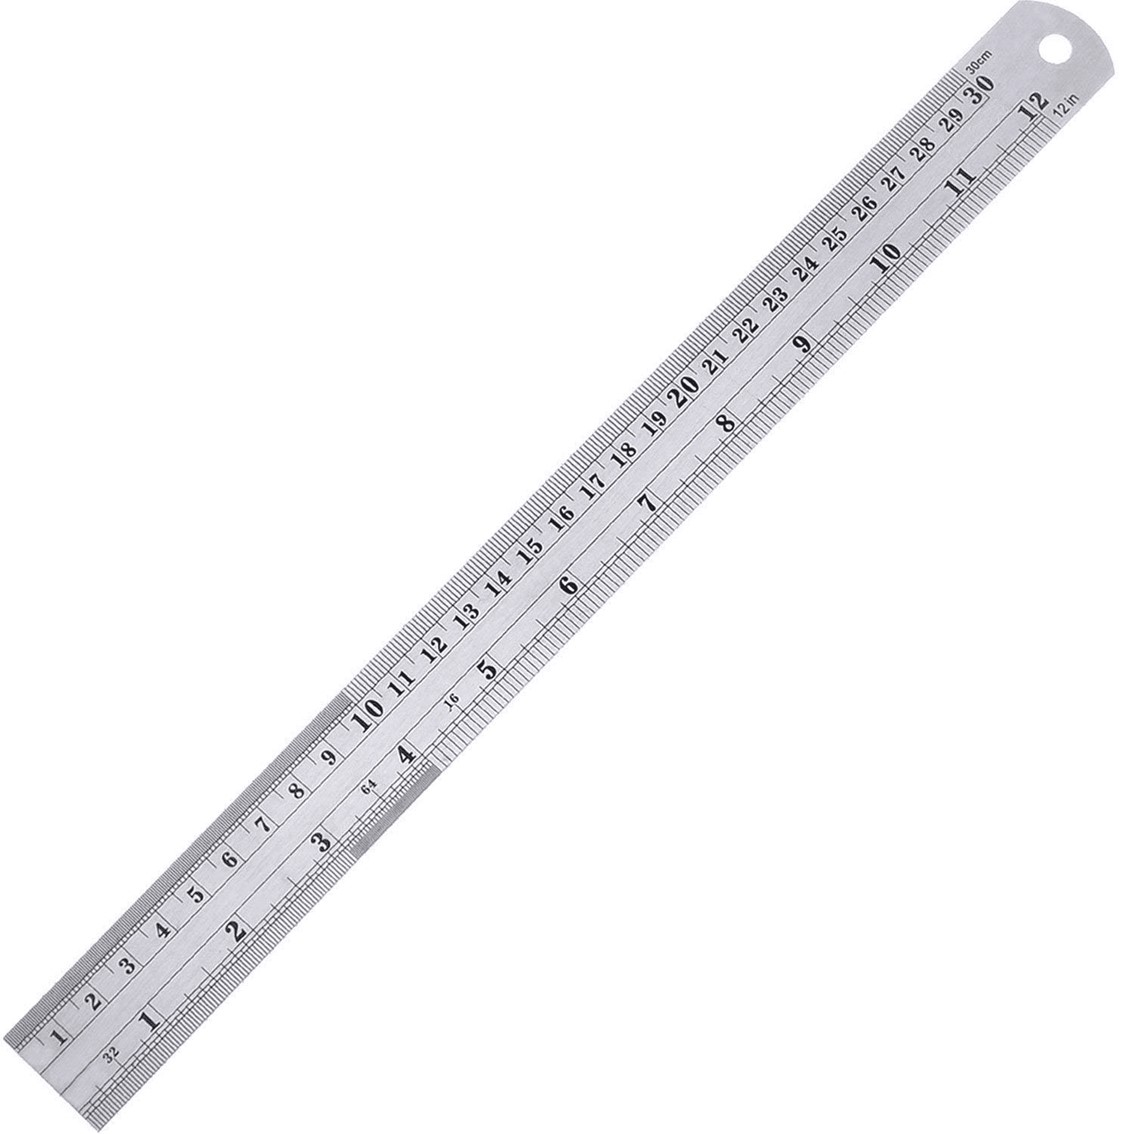
\includegraphics[width = 0.3\textwidth]{Imagenes/regla.jpg}
 		\captionof{figure}{\label{fig:Regla}Regla} 
	\end{center} 
\end{figure}

\begin{figure}[H]
	\begin{center}
 		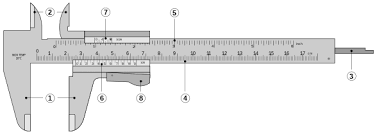
\includegraphics[width = 0.5\textwidth]{Imagenes/vernier.png}
 		\captionof{figure}{\label{fig:pie de rayo  o vernier}pie de rayo  o vernier} 
	\end{center} 
\end{figure}

\subsection{Procedimientos}
\begin{itemize}
    \item Diferenciar entre objeto a medir e instrumentos para medir
    \item Medir las dimensiones del objeto con la regla graduada en milímetros y anotarlas junto al error correspondiente del instrumento.
    \item Medir las dimensiones del objeto con el vernier y anotarlas junto al error correspondiente del instrumento.
    \item Hacer un cuadro que indique las dimensiones, el área y volumen del paralelepípedo medido con la regla y medido con el vernier, indicar sus medidas con su error correspondiente.
    \item suponga que coloca 100 paralepipedo, apoyando uno sobre otro, formando un gran paralepípedo, denotado asi, $A_{100} V_{100}$
\end{itemize}

\subsection{Resultados obtenidos}

\begin{table}[H]
\begin{tabular}{lll}
\cline{1-2}
\multicolumn{1}{|l|}{Incertidumbre de la regla milimetrada:} & \multicolumn{1}{l|}{0,03 cm} &  \\ \cline{1-2}
\multicolumn{1}{|l|}{Incertidumbre del pie de rey:}          & \multicolumn{1}{l|}{0,003}   &  \\ \cline{1-2}
                                                             &                              & 
\end{tabular}
\end{table}



\begin{xltabular}{\textwidth}{|c|c|c|}
    \caption{Medidas con su inceridumbre} \label{tab:long} \\

    \hline \multicolumn{1}{|c|}{} & \multicolumn{1}{c|}{\textbf{Medida de la regla milimetrada}} & \multicolumn{1}{c|}{\textbf{Medida delpie de rey}}  \\ \hline 
    \endfirsthead

    \multicolumn{3}{c}%
    {} \\
    \hline 
    \endhead

    \hline \multicolumn{3}{|r|}{{Continued on next page}} \\ \hline
    \endfoot

    \hline
    \endlastfoot
    Largo (a) & $(3,20 \pm 0,03) cm$                                        & $(3,200 \pm 0,003)cm$                            \\
    Ancho (b) & $(3,19 \pm 0,03)cm$                                        & $(3,195 \pm 0,003)cm$                            \\
    Alto  (h) & $(1,25 \pm 0,03)   cm$                                     & $(1,261 \pm 0,003)cm$                         \\
    Area    (A)      & $(28,90 \pm 0,73)cm^2 $                             & $(29,010 \pm 0,073 )cm^2    $                      \\
    Volumen   (V)       & $(12,76 \pm 0,54)cm^3 $                                 & $(12,892 \pm 0,055)cm^3  $                         \\
    $a_{100}$       & $3,20 \pm 0,03$                                        & $3,200 \pm 0,003               $             \\
    $b_{100}$       & $3,19 \pm 0,03$                                        & $3,195 \pm 0,003          $                  \\
    $h_{100}$       & $125 \pm 3$                                            & $126,1 \pm 0,3 $                             \\
    $A_{100}$       & $1617,92 \pm 53,72$                                    & $1633,267 \pm 4.632 $                        \\
    $V_{100}$       & $1276 \pm 54$                                          & $1289,2 \pm 5,5$            
\end{xltabular}


\begin{itemize}
    \item Cálculo del área total (con la regla)
        \begin{equation*}
            A =2(h)(a+b) + 2(ab)
        \end{equation*}


    \item Cálculo del volumen (con la regla)
        \begin{equation*}
            V = (a)(b)(h) 
        \end{equation*}
        \begin{equation*}
            V=(1,25 \pm 0,03)(3,20 \pm 0,03)(3,19 \pm 0,03)
        = 12,76 \pm 0,54 cm^3
        \end{equation*}


    \item Cálculo de área total (con el pie de rey)
\begin{equation*}
    A=2(h)(a+b) + 2(a)(b) 
\end{equation*}
\begin{equation*}
    A=2(1,261 \pm 0,003)( (3,200 \pm 0,003) + (3,195 \pm 0,003) ) + 2(3,200 \pm 0,003)(3,195 \pm 0,003)
= 29,010 \pm 0,073 cm2
\end{equation*}

    \item Cálculo del volumen (con el pie de rey)
\begin{equation*}
    V=(a)(b)(h)
\end{equation*}
\begin{equation*}
    V=(3,200 \pm 0,003)(3,195 \pm 0,003)(1,261 \pm 0,003)
= 12,892 \pm 0.055 cm3
\end{equation*}

    \item Cálculo de área total de una torre de 100 piezas apiladas 
        \begin{itemize}
            \item Cálculo con regla
    \begin{equation*}
            A_{100}=2(h100)(a+b) + 2(ab)
    \end{equation*}
    \begin{equation*}
        A_{100}=2(125 \pm 3)( (3,20 \pm 0,03) + (3,19 \pm 0,03) ) +2 ( (3,20 \pm 0,03)  (3,19 \pm 0,03) )
        = 1617,92 \pm 53,72 cm2
    \end{equation*}

    \item Cálculo con pie de rey
        \begin{equation*}
            A_{100}=2(h100)(a+b) + 2(ab)
        \end{equation*} 
        \begin{equation*}
            A_{100}=2(126,1 \pm 0,3)( (3,200 \pm 0,003) + (3,195 \pm 0,003) ) + 2(3,200 \pm 0,003)(3,195 \pm 0,003)
        = 1633,267 \pm 4.632 cm2
        \end{equation*}
        \end{itemize}

\end{itemize}

\subsection{Cuestionario}
\begin{enumerate}
    \item \textbf{¿ Las dimensiones de un paralelepípedo se pueden determinar con una sola medición? Si no, ¿ Cuál es el procedimiento más apropiado?}
    
Enfocándonos en la precisión, no sería recomendable realizar una única medición que determine el tamaño de cada lado del paralelepípedo, sino realizar varias mediciones para minimizar el error.
    \item \textbf{¿Qué es más conveniente para calcular el volumen del paralelepípedo: una regla en milímetros o un pie de rey?}

    
Lo más conveniente es el pie de rey debido a su mayor precisión en la medición, en la graduación y la forma de medir, de modo que al calcular el volumen la incertidumbre es mucho menor que con una regla.

\end{enumerate}